\chapter{Implementation and Results}

This chapter describes how the system is being developed, the work completed so far, the testing carried out, and the results obtained. The results reported here are measured on the actual code base; no figures are estimated.

\section{Development Approach}
The project started from a hackathon prototype that already contained many screens and a large database schema. A detailed audit of the prototype (described in Section~\ref{sec:audit}) showed that much of what appeared to work was driven by hard-coded demonstration data. Rather than adding features on top of this, the work was organised into eight phases, each ending in something that works and can be demonstrated, and each pushed to its own branch of the project's Git repository. Figure~\ref{fig:gantt} shows the plan.

\begin{figure}[H]
\centering
\begin{ganttchart}[
  hgrid,vgrid,
  x unit=0.68cm,
  y unit chart=0.62cm,
  bar height=0.55,
  bar/.append style={fill=nexusblue!35,draw=nexusblue},
  milestone/.append style={fill=nexusgreen},
  title label font=\scriptsize\bfseries,
  bar label font=\scriptsize,
  title height=1,
]{1}{12}
\gantttitle{Week}{12} \\
\gantttitlelist{1,...,12}{1} \\
\ganttbar[bar/.append style={fill=nexusgreen!55,draw=nexusgreen}]{Phase 0: Clean-up \& security fixes}{1}{2} \\
\ganttbar{Phase 1: Schema, regions, real auth}{3}{4} \\
\ganttbar{Phase 2: Lifecycle core \& ledger}{4}{5} \\
\ganttbar{Phase 3: Proposals, funding, milestones}{6}{7} \\
\ganttbar{Phase 4: Closure, credentials, scores}{8}{8} \\
\ganttbar{Phase 5: Seed data \& tests}{9}{9} \\
\ganttbar{Phase 6: Design \& screens}{9}{11} \\
\ganttbar{Phase 7: Documentation \& deployment}{12}{12} \\
\ganttbar[bar/.append style={fill=nexusamber!45,draw=nexusamber}]{Report \& presentations}{2}{12}
\end{ganttchart}
\caption{Phase-wise development plan (green: completed)}
\label{fig:gantt}
\end{figure}

\begin{table}[H]
\centering
\caption{Development phases and their completion criteria}
\label{tab:phases}
\small
\begin{tabularx}{\textwidth}{@{}p{1.3cm}p{4.4cm}Xp{1.7cm}@{}}
\toprule
\textbf{Phase} & \textbf{Work} & \textbf{Done when} & \textbf{Status} \\
\midrule
0 & Remove dead code and fabricated data; fix live security, integrity and privacy defects & Unknown IDs return 404; build passes; integrity tests pass & Completed \\
1 & New schema with Indian states/districts; real authentication; role guards & Every role signs in for real; wrong role receives 403 & In progress \\
2 & Lifecycle service, ledger, notifications; reporting, verification, endorsements, priority queue & A report moves to OPEN FOR PROPOSALS through the API with ledger entries & Planned \\
3 & Proposals with teams and milestones; selection; CSR co-funding; proof upload; tranche release & Demonstration case reaches COMPLETED with money matching milestones & Planned \\
4 & Citizen confirmation/dispute; credentials with QR; impact scores; daily job & Demonstration case reaches RESOLVED; tampering is detected & Planned \\
5 & Deterministic demonstration data and automated checks & Seed and checks pass from an empty database & Planned \\
6 & Design system and all role screens; India map & Every screen works with real data on desktop and mobile & Planned \\
7 & Documentation; fresh deployment & Demonstration runs end to end on the deployed site & Planned \\
\bottomrule
\end{tabularx}
\end{table}

\section{Audit of the Prototype}\label{sec:audit}
The prototype was audited in three ways: by reading all 231 tracked source files, by reviewing the public deployment, and by signing in as each demonstration role on a local copy and exercising every screen. The most important findings are summarised below.

\begin{itemize}
  \item \textbf{Fabricated responses.} Many API routes returned built-in demonstration data whenever a record was not found or the database was unavailable. As a result, \emph{any} made-up credential identifier was displayed as ``verified'', and tracking an unknown challenge identifier showed a different, invented challenge. Both behaviours were confirmed on the public deployment.
  \item \textbf{False success.} Submitting a report, routing a challenge or issuing credentials displayed a success message even when nothing had been saved, and a failed project submission silently discarded the user's input.
  \item \textbf{Wrong-record defects.} When an identifier was not found, some routes acted on a different record instead: the matching service used the oldest challenge in the database, credential issuing used the first student profile, and milestone submission attached proof to the first project team.
  \item \textbf{Integrity defects.} Milestone hashes were computed from a timestamp different from the stored one, so every genuine milestone would have failed verification, while the verification route trusted a hash supplied by the browser.
  \item \textbf{Permission defects.} A university could mark its own proposal as accepted, milestones could jump to any status, and students received the faculty's actions.
  \item \textbf{Privacy defects.} Users without notifications were shown other users' notifications, a public list exposed reporters' phone numbers, the public credential API returned the student's e-mail address, and avatar images sent users' e-mail addresses to a third-party service.
  \item \textbf{Crash and inconsistencies.} One government dashboard tab crashed because the page and its API expected different data shapes, and the same totals (such as the number of challenges or organisations) differed between screens because each screen used its own hard-coded data.
\end{itemize}

\section{Implementation of Phase 0}
Phase~0 removed the causes of these findings and cleaned the code base before new features are built on it. Its main changes were:
\begin{enumerate}
  \item Every lookup by identifier now returns \emph{not found} (HTTP 404) for an unknown record and \emph{temporarily unavailable} (HTTP 503) when the database cannot be reached. All built-in fallback datasets were removed from the API and from the pages.
  \item Credential and ledger verification now recompute hashes only from stored data; milestone submission hashes exactly the values it stores; a milestone without a stored hash is reported as not verifiable.
  \item Proposal and milestone status changes follow explicit allowed transitions; universities can only save drafts or submit; credential issuing requires every milestone to be approved, issues credentials to all listed students or none, prevents duplicates and caps hours.
  \item Team formation accepts only students of the faculty member's own university and writes the team and the status change in one transaction.
  \item Notifications are scoped to the requesting user; personal data was removed from public responses; avatars are generated locally from initials.
  \item The duplicate-detection service was re-implemented without an external natural-language library, computing TF-IDF weights from the district's own reports.
  \item Fifty-five unused API routes, the unused donor role, eight unused services, twelve demonstration scripts and seven unused packages were removed, and all region-specific hackathon wording was replaced.
\end{enumerate}

Table~\ref{tab:phase0} quantifies the result.

\begin{table}[H]
\centering
\caption{Measured effect of Phase 0 on the code base}
\label{tab:phase0}
\small
\begin{tabular}{@{}lrr@{}}
\toprule
\textbf{Measure} & \textbf{Before} & \textbf{After} \\
\midrule
API route files & 103 & 34 \\
Source files under \texttt{src/} & 199 & 111 \\
Files changed in Phase 0 & \multicolumn{2}{r}{168} \\
Lines added / removed & \multicolumn{2}{r}{2{,}306 / 14{,}329} \\
Routes returning fabricated fallback data & many & 0 \\
Production build warnings & present & 0 \\
Automated integrity tests passing & -- & 6 of 6 \\
\bottomrule
\end{tabular}
\end{table}

\section{Testing}
Following the project's rule that every non-trivial piece of logic leaves behind a small runnable check, Phase~0 added an integrity test file executed with the Node.js built-in test runner (\texttt{npm run check}). Table~\ref{tab:tests} lists the tests and their results.

\begin{table}[H]
\centering
\caption{Integrity tests and results}
\label{tab:tests}
\small
\begin{tabularx}{\textwidth}{@{}p{0.6cm}Xp{1.4cm}@{}}
\toprule
\textbf{No.} & \textbf{Test (what must hold)} & \textbf{Result} \\
\midrule
1 & The hash stored at milestone submission equals the hash recomputed at verification, with and without proof and GPS & Pass \\
2 & Changing the proof, a coordinate or the timestamp by one millisecond changes the hash & Pass \\
3 & A credential hash is deterministic and changes when the credits change & Pass \\
4 & Credits follow the rule of 30 verified hours per whole credit & Pass \\
5 & A project with no milestones, or with any unapproved milestone, is not complete & Pass \\
6 & Duplicate detection scores a reworded duplicate above an unrelated report & Pass \\
\bottomrule
\end{tabularx}
\end{table}

In addition, each change was checked by a full TypeScript type check and a production build, both of which complete without errors or warnings, and by exercising the affected pages in a browser. With the database disconnected, the credential verification page for a made-up identifier now shows ``Credential Not Found'' with the reason, instead of the previous ``Verified'' badge, and the government dashboard's policy-insights tab shows an explanatory message instead of crashing.

\section{Result Analysis: Duplicate Detection}
To evaluate the duplicate-detection rule, a new report was compared with four existing reports from the same village using the implemented TF-IDF cosine similarity. Table~\ref{tab:dedup} shows the measured similarities.

\begin{table}[H]
\centering
\caption{Duplicate-detection experiment}
\label{tab:dedup}
\small
\begin{tabularx}{\textwidth}{@{}Xrp{2.6cm}@{}}
\toprule
\multicolumn{3}{@{}l}{\textbf{New report:} ``High fluoride in borewell drinking water, children have dental fluorosis''} \\
\midrule
\textbf{Existing report} & \textbf{Similarity} & \textbf{Decision at 0.75} \\
\midrule
A. ``Borewell water in our village has high fluoride; kids show fluorosis'' (same problem, reworded) & 0.535 & not flagged \\
B. ``Drinking water pipeline leaks near the school, supply is irregular'' (same village, related topic) & 0.177 & not flagged \\
C. ``Village road floods every monsoon and cuts off the health centre'' & 0.000 & not flagged \\
D. ``Primary school has no working toilets for girls'' & 0.000 & not flagged \\
\bottomrule
\end{tabularx}
\end{table}

The method separates the genuine duplicate (A) clearly from the related but different report (B) and from unrelated reports (C, D). However, with the prototype's threshold of 0.75 even the genuine duplicate is not flagged, because a citizen rewording the problem (``kids'' instead of ``children'', ``fluorosis'' instead of ``dental fluorosis'') shares only part of the vocabulary. This result motivated the design described in Section~\ref{sec:dedup}: a lower similarity threshold of 0.5 combined with a requirement that the existing challenge is in the same category and within 2\,km, so that recall improves while the distance check keeps unrelated reports from other places from being matched. The citizen always makes the final choice between endorsing the existing report and submitting a new one.

\section{User Interface}
Figures~\ref{fig:ui-landing} and \ref{fig:ui-report} show two screens of the current prototype after Phase~0. The visual design of all screens is redesigned in Phase~6 using a consistent design system; screenshots of the final role workspaces will replace these in the final version of the report.

\begin{figure}[H]
\centering

\includegraphics[width=0.92\textwidth]{figures/ui-landing.png}
\caption{Landing page of the prototype}
\label{fig:ui-landing}
\end{figure}

\begin{figure}[H]
\centering
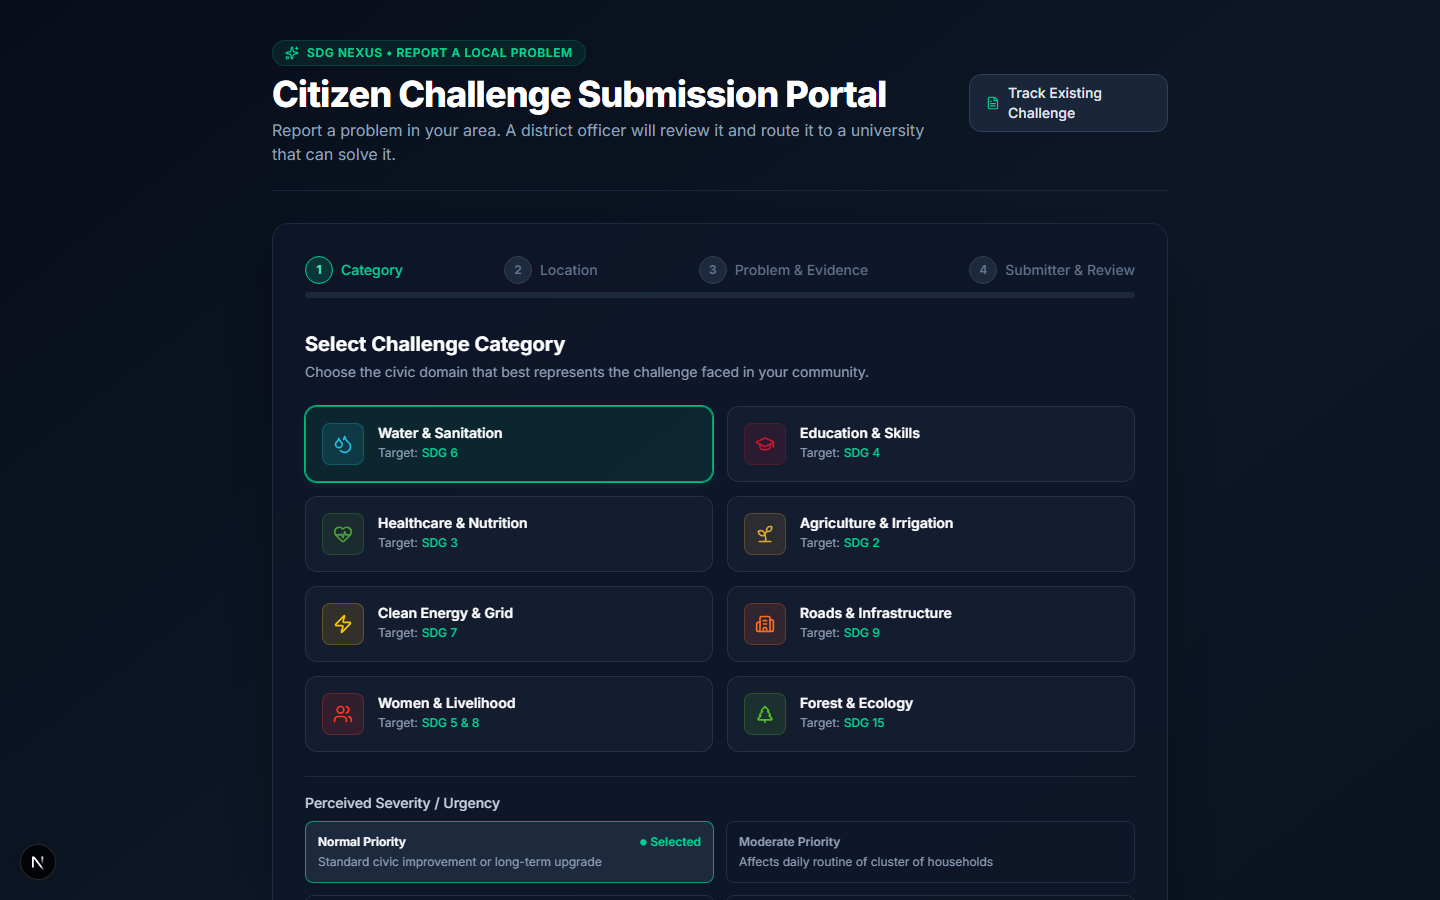
\includegraphics[width=0.92\textwidth]{figures/ui-report.png}
\caption{Citizen problem-report form (step 1: category and urgency)}
\label{fig:ui-report}
\end{figure}

\section{Innovation}
SDG Nexus introduces the following contributions:
\begin{itemize}
  \item \textbf{A citizen-closed loop.} The same citizen who reports a problem confirms (or disputes) the solution, and that confirmation feeds both the students' credentials and the organisations' impact scores. No reviewed platform closes this loop.
  \item \textbf{Money that follows proof.} Milestone amounts must add up to the budget, and each tranche can be released only after its milestone is verified, enforced inside a database transaction rather than by convention.
  \item \textbf{Server-governed lifecycle.} A single state machine on the server decides which actions are possible and returns them to the interface, so buttons cannot appear for actions that are not allowed, and every transition writes its ledger entry and notifications atomically.
  \item \textbf{Tamper evidence without a blockchain.} A per-challenge SHA-256 hash chain and server-side hashing of proof files let anyone verify the full history, at a fraction of the cost and complexity of a blockchain.
  \item \textbf{Endorsements instead of duplicates.} Repeated reports of the same problem become a measured demand signal that raises the challenge's priority instead of cluttering the officer's queue.
  \item \textbf{Explainable automation.} Priority, matching and duplicate detection are transparent formulas whose components are shown to the user, so that officers can trust and override them.
  \item \textbf{Honest by construction.} The platform never substitutes demonstration data for missing records and never reports success for an action that was not saved, a property verified by the audit and the tests above.
\end{itemize}
